\documentclass[11pt,a4paper,oneside]{report}
\usepackage{iftex}
\ifPDFTeX
  \usepackage[T1]{fontenc}
\fi
\usepackage[czech]{babel}
\usepackage[margin=28mm]{geometry}
\usepackage{tikz}
\usetikzlibrary{babel,shapes.geometric,arrows.meta}
\tikzset{
  aktivita/.style={font=\small,align=center},
  krok/.style={draw,rounded corners=3pt,fill=white,inner sep=5pt},
  volba/.style={diamond,draw,inner sep=0pt,minimum size=5mm},
  tok/.style={-{Stealth[length=2mm]}},
  start/.style={circle,fill,inner sep=0pt,minimum size=3mm},
  konec/.style={circle,draw,double=white,double distance=1pt,fill=black,inner sep=0pt,minimum size=3.5mm}
}

\begin{document}
\begin{titlepage}
\vspace*{0.24\textheight}
\begin{center}
    {\large Vývoj informačních systémů\par}
    \medskip
    {\LARGE Informační systém pro řízení zásob a plánování jídel
    v gastronomickém provozu\par}
\end{center}
\end{titlepage}

\chapter{Vize}

Systém slouží k~evidenci zásob a~plánování jídel v~gastronomickém provozu.
U~surovin eviduje množství na skladě a~datum spotřeby. Podle zásob
a~uložených receptů vypočítá, kolik porcí jednotlivých jídel lze připravit.
Přednostně doporučí jídla, která využijí suroviny s~blížícím se datem spotřeby.

Pro denní plán jídel sestaví nákupní seznam chybějících surovin.
Po potvrzení přípravy odečte spotřebované množství ze skladu.
\chapter{Funkční specifikace}

\section{Aktéři a případy užití}

Pracovník kuchyně eviduje suroviny, sleduje zásoby a~potvrzuje přípravu jídel.
Vedoucí kuchyně spravuje recepty a~rozhoduje, která jídla a~v~jakém množství
zařadí do denního plánu. Obě role může zastávat stejná osoba.

\begin{figure}[htbp]
\centering
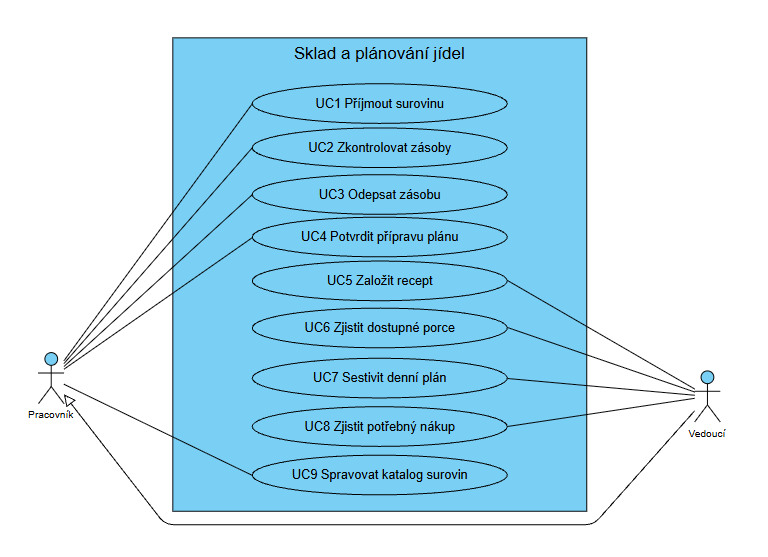
\includegraphics[width=\linewidth,height=.60\textheight,keepaspectratio]{diagramy/VIS Use Case.png}
\caption{Případy užití a~jejich hlavní aktéři.}
\end{figure}

\section{Popis případů užití}

\paragraph{UC1 -- Přijmout surovinu.}
Pracovník vybere surovinu, zadá přijaté množství a~datum spotřeby.
Systém uloží příjem jako samostatnou skladovou položku. U~nové suroviny
pracovník doplní kategorii a~jednotku. Systém ji při příjmu zařadí
do katalogu. Přijaté množství musí být kladné.

\paragraph{UC2 -- Zkontrolovat zásoby.}
Pracovník otevře přehled skladu. U~každé dostupné suroviny vidí součet
použitelného množství. Přehled zvlášť uvádí suroviny s~kladným zůstatkem
pod nastaveným minimem a~skladové položky, kterým datum spotřeby
připadne na dnešek nebo na některý z~následujících tří dnů.

\paragraph{UC3 -- Odepsat zásobu.}
Při spotřebě mimo denní plán nebo při vyřazení suroviny pracovník vybere
konkrétní skladovou položku a~zadá množství. Systém sníží její zůstatek.
Při úplném odepsání položku odstraní ze skladu. Pokud zadané množství
přesáhne zůstatek, systém zápis odmítne.

\paragraph{UC4 -- Potvrdit přípravu plánu.}
Pracovník vybere uložený plán a~potvrdí přípravu všech jeho jídel.
Systém sečte potřebná množství a~odepíše je ze zásob použitelných
v~den potvrzení, počínaje nejbližším datem spotřeby. Poté označí plán
jako připravený. Chybí-li některá surovina, stav skladu i~plánu zůstane
beze změny. Již připravený plán nelze potvrdit podruhé.

\paragraph{UC5 -- Založit recept.}
Vedoucí zadá název jídla, postup, počet porcí a~množství každé suroviny
pro celý recept. Může vybrat surovinu z~katalogu nebo zadat novou,
i~když ještě není na skladě. Po uložení je recept k~dispozici pro plánování.
Recept musí obsahovat alespoň jednu surovinu.

\paragraph{UC6 -- Zjistit dostupné porce.}
Vedoucí zvolí den přípravy. Systém pro každý recept porovná množství
potřebné na porci se zásobami použitelnými ve zvolený den. Počet celých
porcí určí surovina, která vystačí na nejméně porcí. Výsledek platí
pro každý recept zvlášť. Přednost dostanou proveditelné recepty,
které využijí surovinu s~blížícím se datem spotřeby.

\paragraph{UC7 -- Sestavit denní plán.}
Vedoucí vybere den, alespoň jeden recept a~kladný počet porcí pro každé
jídlo. Systém uloží jeden plán pro daný den. Stejný recept smí být v~plánu
jen jednou. Plán může počítat i~se surovinami, které je třeba dokoupit.
Uložením plánu se zásoby nemění.

\paragraph{UC8 -- Zjistit potřebný nákup.}
Vedoucí vybere uložený plán. Systém sečte potřebu každé suroviny
napříč všemi plánovanými jídly a~porovná ji se zásobou použitelnou
v~den plánu. Nákupní seznam obsahuje pouze chybějící množství.
Pokud zásoby stačí nebo je plán již připravený, seznam je prázdný.

\paragraph{UC9 -- Spravovat katalog surovin.}
Pracovník zvolí provozní katalog nebo samostatný seznam CSV. Při přidání
suroviny zadá název, kategorii, jednotku a~minimální zásobu. Podle potřeby
může založit novou kategorii. Pro sklad, recepty a~plánování se používají
suroviny z~provozního katalogu.

\section{Diagramy aktivit}

\begin{figure}[htbp]
\centering
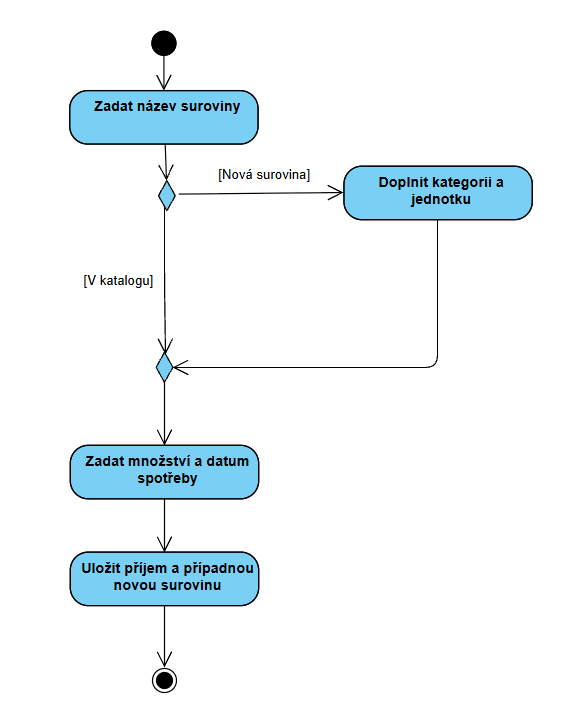
\includegraphics[width=\linewidth,height=.60\textheight,keepaspectratio]{diagramy/VIS Activity 1.png}
\caption{Příjem suroviny na sklad (UC1).}
\end{figure}

\begin{figure}[htbp]
\centering
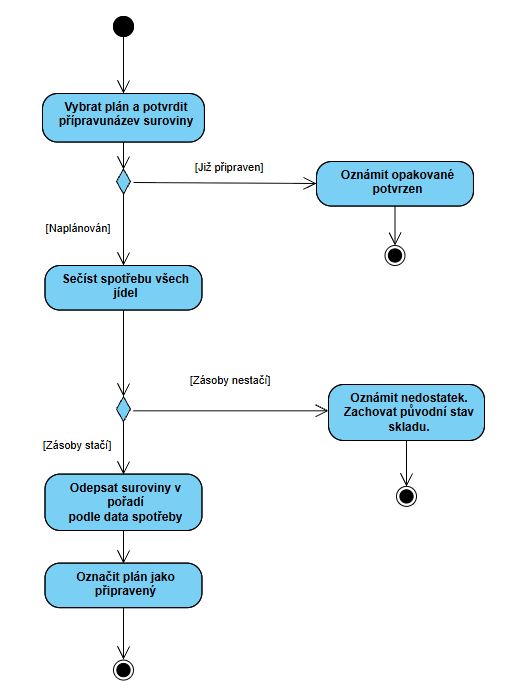
\includegraphics[width=\linewidth,height=.60\textheight,keepaspectratio]{diagramy/VIS Activity 2.png}
\caption{Potvrzení přípravy denního plánu (UC4).}
\end{figure}
\chapter{Technická specifikace}

\section{První model domény}

Surovina má v~katalogu název, kategorii, měrnou jednotku a~minimální
zásobu. Každý příjem na sklad zakládá samostatnou skladovou položku
se zbývajícím množstvím a~datem spotřeby. Dvě balení mléka s~různými
daty spotřeby tak patří ke stejné surovině, ale lze je odepisovat zvlášť.

\begin{figure}[htbp]
\centering
\begin{tikzpicture}[font=\small,
  pojem/.style={draw,align=center,minimum width=3.5cm,minimum height=.9cm},
  pocet/.style={font=\footnotesize,inner sep=2pt}]
  \node[pojem] (cat) at (0,0) {Kategorie};
  \node[pojem] (ing) at (5,0) {Surovina};
  \node[pojem] (stock) at (10,0) {Skladová položka};
  \node[pojem] (line) at (5,-2) {Surovina v~receptu};
  \node[pojem] (recipe) at (10,-2) {Recept};
  \node[pojem] (planline) at (10,-4) {Položka plánu};
  \node[pojem] (plan) at (5,-4) {Denní plán};
  \draw (cat)--node[pocet,at start,anchor=south west]{1}
    node[pocet,at end,anchor=south east]{0..*}(ing);
  \draw (ing)--node[pocet,at start,anchor=south west]{1}
    node[pocet,at end,anchor=south east]{0..*}(stock);
  \draw (ing)--node[pocet,at start,anchor=north west]{1}
    node[pocet,at end,anchor=south west]{0..*}(line);
  \draw (line)--node[pocet,at start,anchor=south west]{1..*}
    node[pocet,at end,anchor=south east]{1}(recipe);
  \draw (recipe)--node[pocet,at start,anchor=north west]{1}
    node[pocet,at end,anchor=south west]{0..*}(planline);
  \draw (plan)--node[pocet,at start,anchor=south west]{1}
    node[pocet,at end,anchor=south east]{1..*}(planline);
\end{tikzpicture}
\caption{Doménové pojmy a~počet jejich výskytů ve vztahu.}
\end{figure}

Recept určuje postup a~základní počet porcí. Každá surovina v~receptu
má uvedené množství pro tento počet porcí v~jednotce z~katalogu.
Denní plán patří jednomu dni. Každá jeho položka odkazuje na jeden
recept a~určuje, kolik porcí se má připravit. Plán eviduje také to,
zda už kuchyně přípravu potvrdila.

\section{Volba technologií a pracovních postupů}

\paragraph{Uložení dat.}
Recepty i~sklad odkazují na stejné suroviny. PostgreSQL tyto vazby
hlídá pomocí cizích klíčů a~umožňuje spojit recept s~názvy a~množstvím
surovin jedním SQL dotazem. Katalog surovin podporuje také uložení
do souboru CSV. Třída \texttt{IngredientDaoFactory} vybírá mezi dvěma
implementacemi stejného rozhraní. Sklad, recepty a~denní plány používají
PostgreSQL.

\paragraph{Zpracování požadavků.}
Uživatelské rozhraní tvoří stránka v~HTML, CSS a~JavaScriptu. Při potvrzení
přípravy odešle identifikátor plánu na server. Serverová část v~Javě~21
používá Spring Boot. Kontroler převezme požadavek a~předá ho službě,
která řídí přípravu. Jednotlivé DAO čtou a~zapisují data pomocí JDBC
a~přímo zadaných SQL dotazů. Výpočet spotřeby tak lze použít i~pro
sestavení nákupního seznamu.

\paragraph{Výpočet porcí a odpis zásob.}
Pro každou surovinu systém přepočte použitelné zásoby na počet celých
porcí podle receptu. Výsledek určuje surovina, která vystačí na nejméně
porcí. U~denního plánu se naopak vychází z~požadovaného počtu porcí
a~spotřeba stejné suroviny se sečte přes všechna jídla. Výpočet používá
desetinný typ \texttt{BigDecimal}. Součet se zaokrouhlí jednou pro každou
surovinu, takže nákupní seznam i~odpis vycházejí ze stejného množství.

Při potvrzení plánu služba odepisuje nejprve zásoby s~nejbližším datem
spotřeby. Odpisy a~označení plánu jako připraveného proběhnou v~jedné
databázové transakci. Pokud například až u~poslední suroviny zásoba
nestačí, databáze vrátí i~předchozí odpisy tohoto plánu.
\chapter{Skica uživatelského rozhraní}

\begin{center}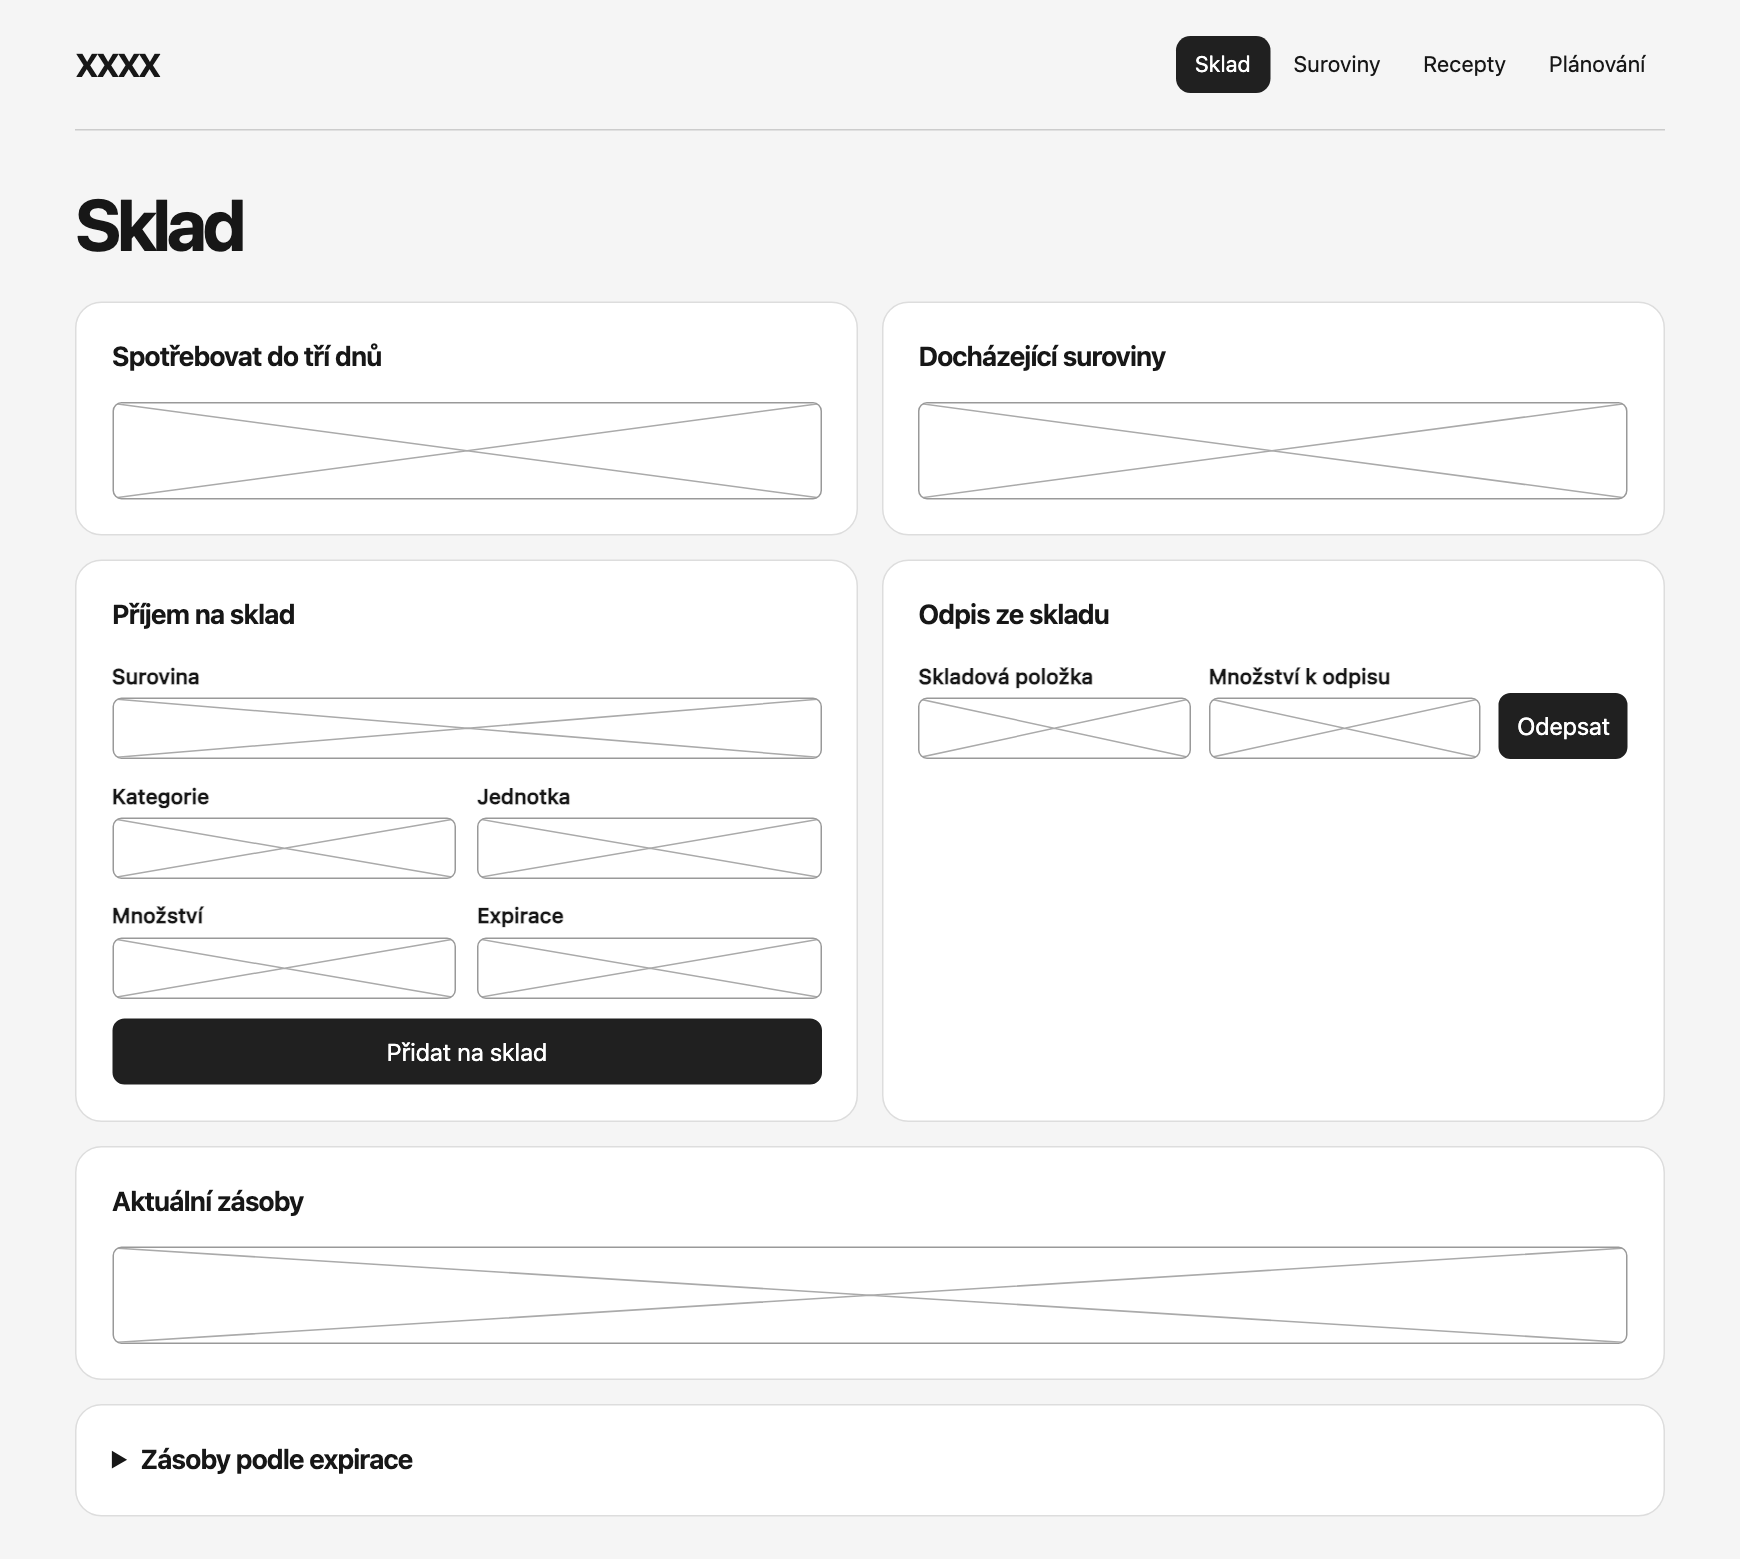
\includegraphics[width=\linewidth]{wireframy/sklad.png}\end{center}
\clearpage
\begin{center}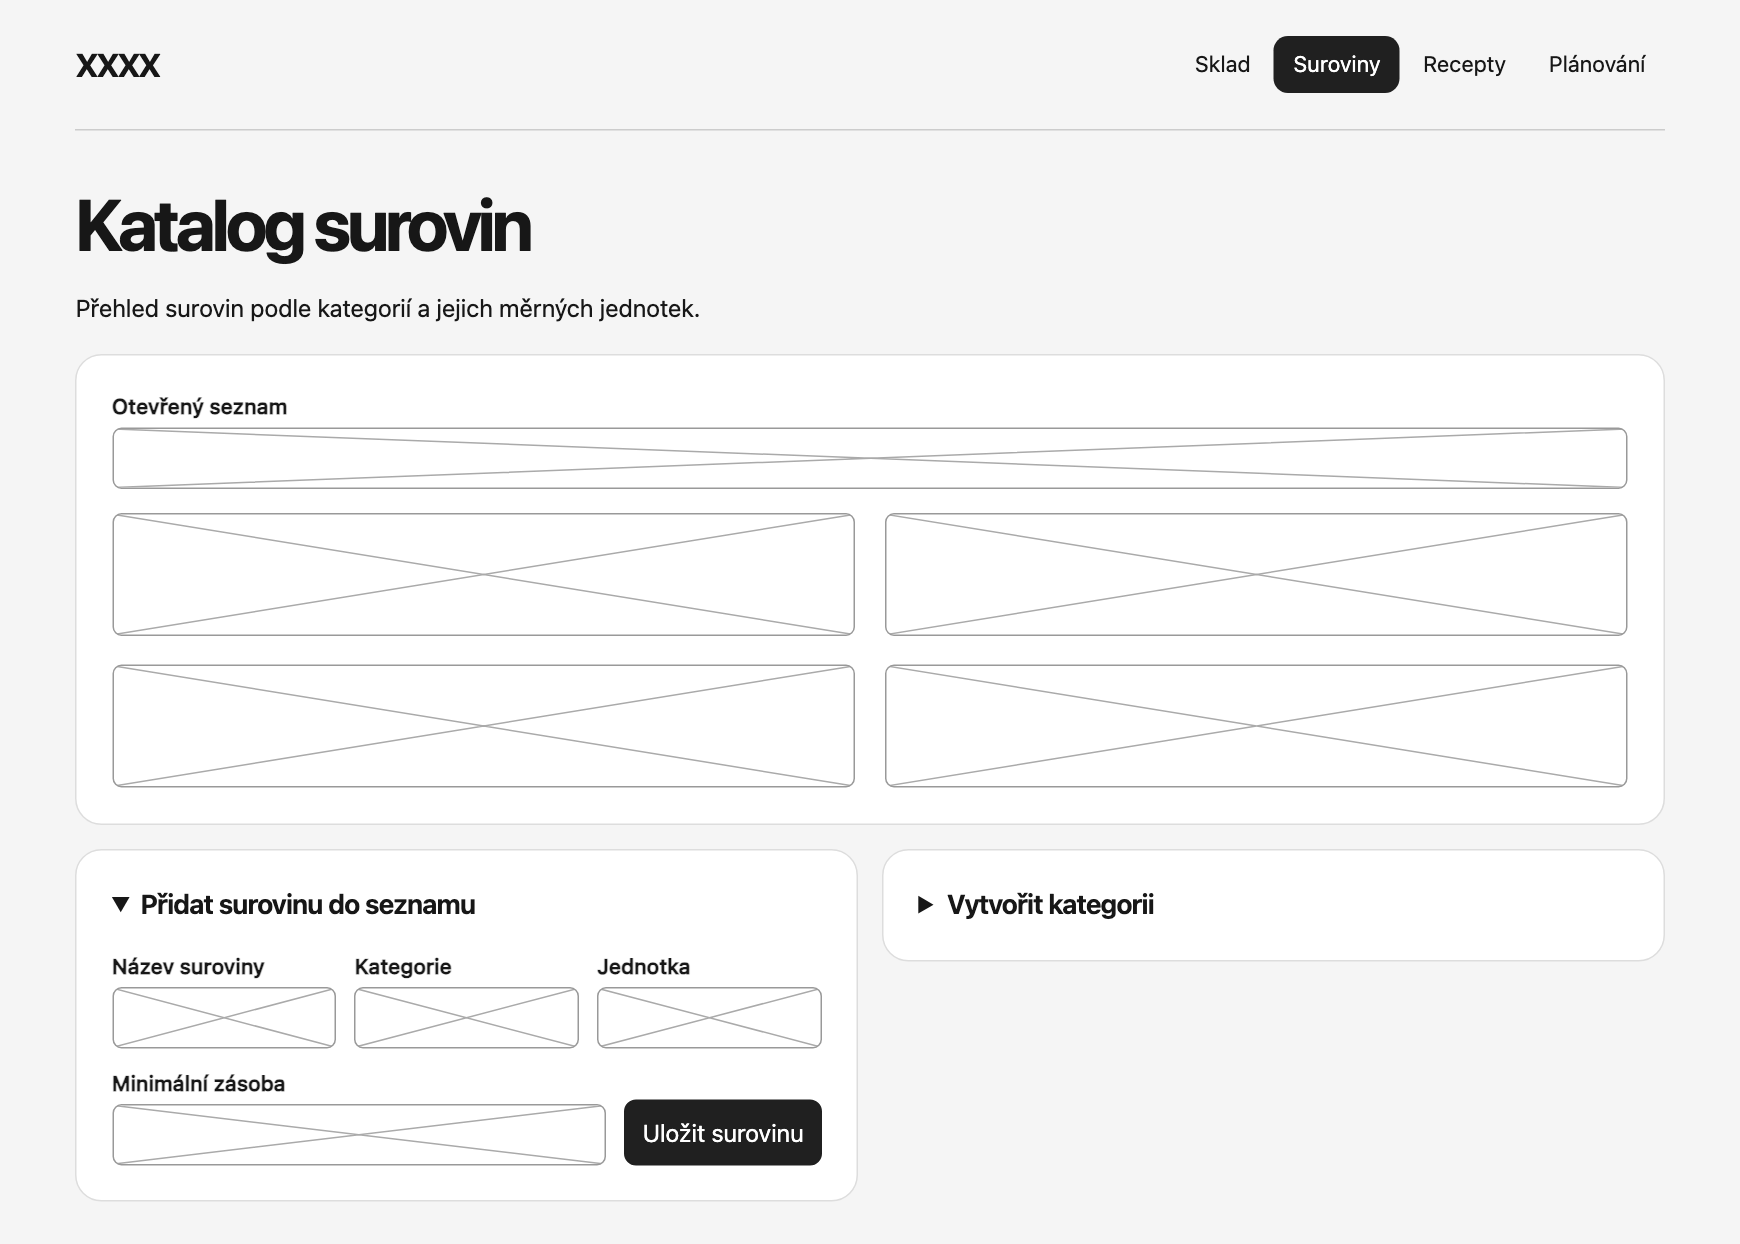
\includegraphics[width=\linewidth]{wireframy/suroviny.png}\end{center}

\clearpage
\begin{center}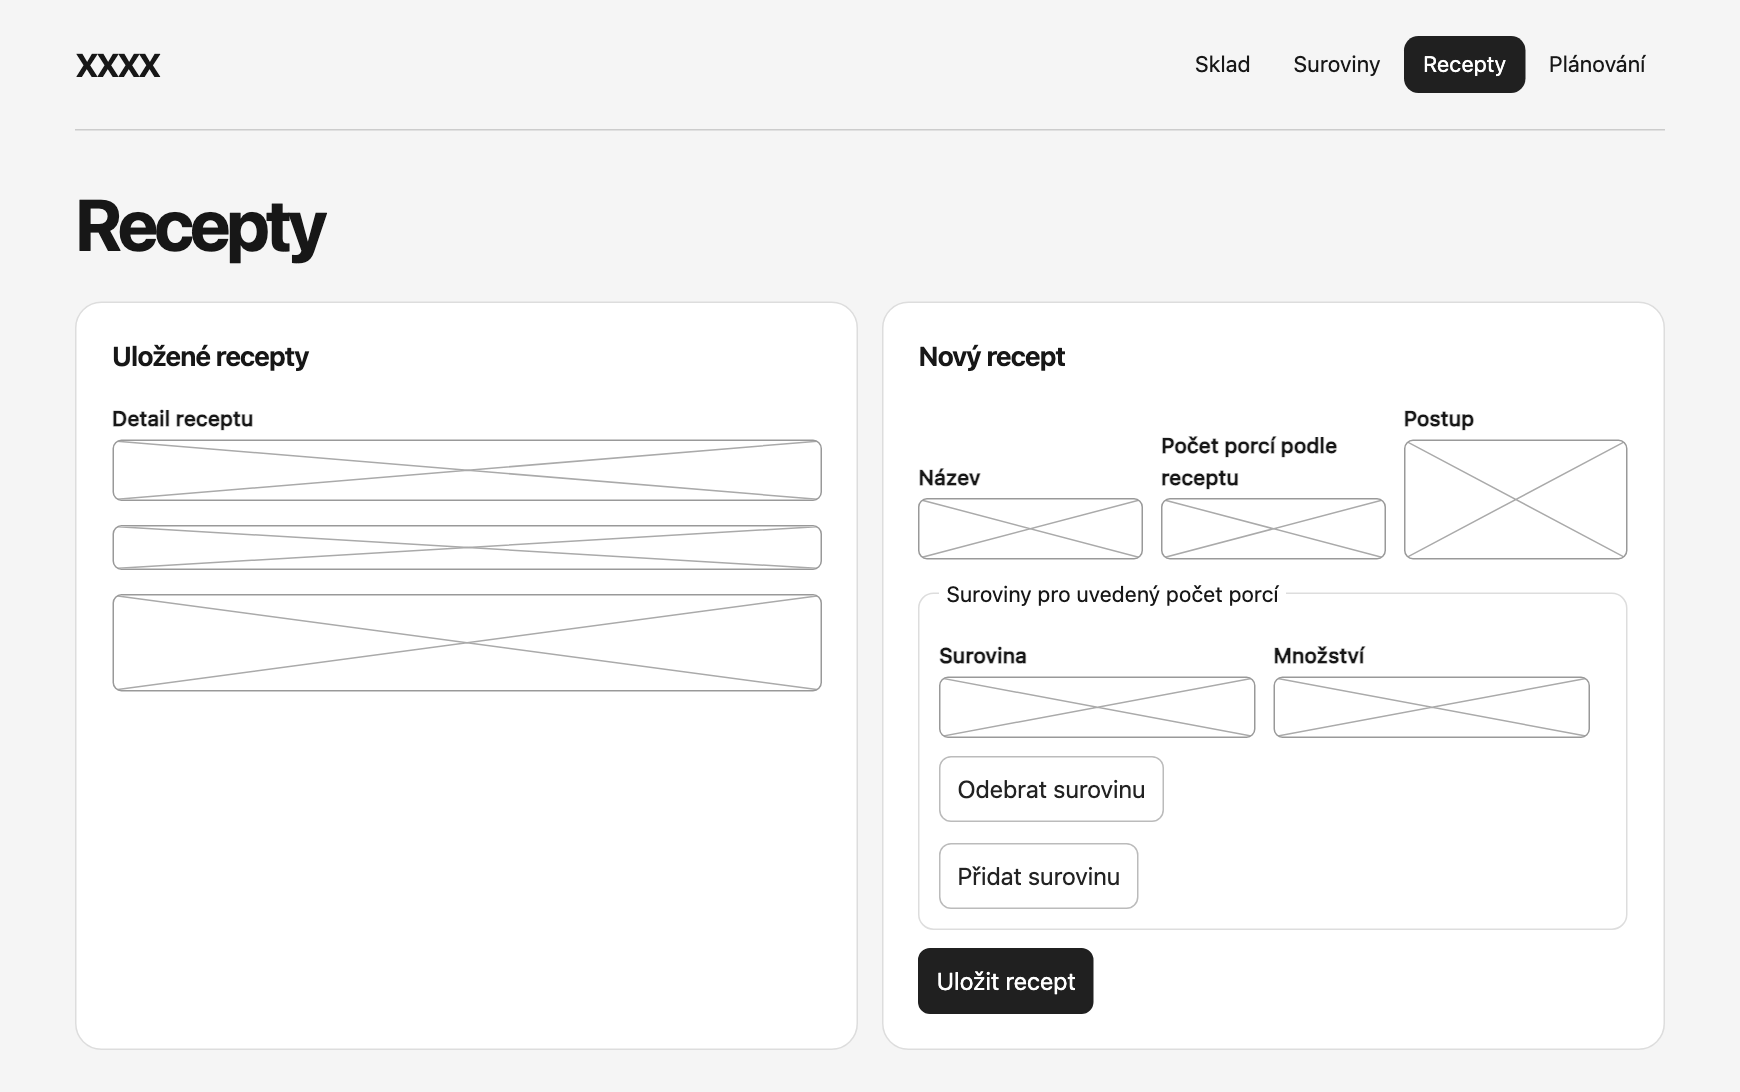
\includegraphics[width=\linewidth]{wireframy/recepty.png}\end{center}
\clearpage
\begin{center}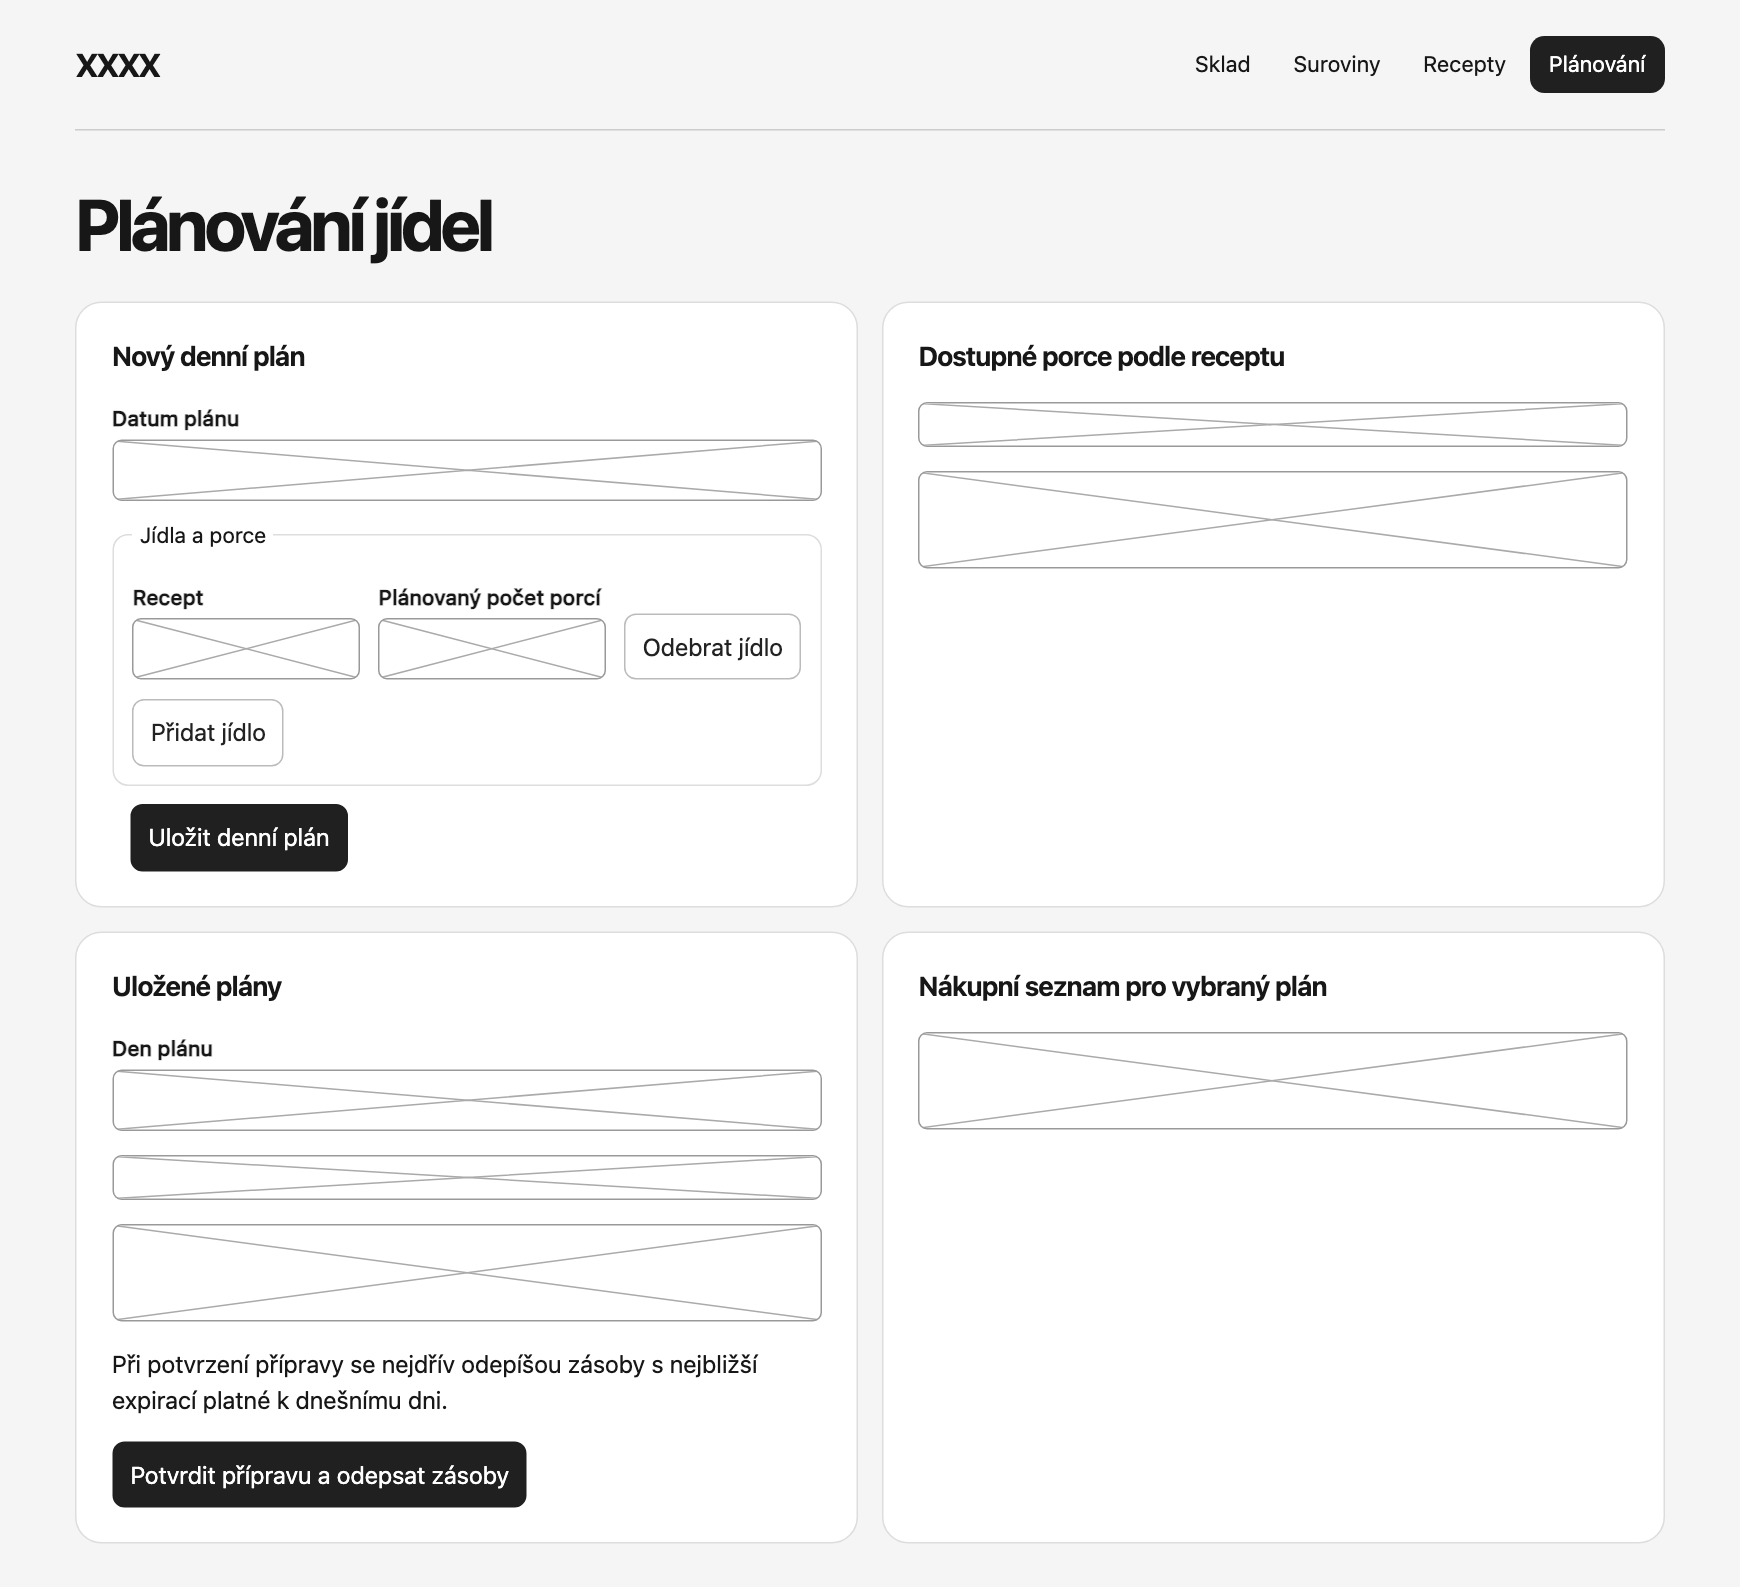
\includegraphics[width=\linewidth]{wireframy/planovani.png}\end{center}
\chapter{Návrh doménového modelu}
\section{Statický diagram tříd}
Model tvoří datové třídy z~balíčku \texttt{cz.rest.model}, zapsané
v~Javě jako \texttt{record}. Čáry znázorňují vazby uložené pomocí
identifikátorů. Například \texttt{Delivery.ingredientId} určuje, ke které
surovině skladová položka patří.

\begin{center}
\begin{tikzpicture}[font=\small,box/.style={draw,fill=white,inner sep=0pt}]
\node[box] (Category) at (0,0) {\begin{tabular}{l}\multicolumn{1}{c}{\bfseries Category}\\\hline
\texttt{Long id}\\
\texttt{String name}\end{tabular}};
\node[box] (Ingredient) at (5,0) {\begin{tabular}{l}\multicolumn{1}{c}{\bfseries Ingredient}\\\hline
\texttt{Long id}\\
\texttt{String name}\\
\texttt{Long categoryId}\\
\texttt{String unit}\\
\texttt{BigDecimal minimum}\end{tabular}};
\node[box] (Delivery) at (10,0) {\begin{tabular}{l}\multicolumn{1}{c}{\bfseries Delivery}\\\hline
\texttt{Long id}\\
\texttt{Long ingredientId}\\
\texttt{BigDecimal remaining}\\
\texttt{LocalDate expires}\end{tabular}};
\node[box] (RecipeLine) at (5,-4) {\begin{tabular}{l}\multicolumn{1}{c}{\bfseries RecipeLine}\\\hline
\texttt{long ingredientId}\\
\texttt{BigDecimal quantity}\end{tabular}};
\node[box] (Recipe) at (10,-4) {\begin{tabular}{l}\multicolumn{1}{c}{\bfseries Recipe}\\\hline
\texttt{Long id}\\
\texttt{String name}\\
\texttt{String instructions}\\
\texttt{int servings}\end{tabular}};
\node[box] (MealPlan) at (5,-7.8) {\begin{tabular}{l}\multicolumn{1}{c}{\bfseries MealPlan}\\\hline
\texttt{long id}\\
\texttt{LocalDate day}\\
\texttt{boolean prepared}\end{tabular}};
\node[box] (PlanLine) at (10,-7.8) {\begin{tabular}{l}\multicolumn{1}{c}{\bfseries PlanLine}\\\hline
\texttt{long recipeId}\\
\texttt{int portions}\end{tabular}};
\draw (Category)--node[at start,anchor=south west,font=\footnotesize]{1} node[at end,anchor=south east,font=\footnotesize]{0..*}(Ingredient);
\draw (Ingredient)--node[at start,anchor=south west,font=\footnotesize]{1} node[at end,anchor=south east,font=\footnotesize]{0..*}(Delivery);
\draw (Ingredient)--node[at start,anchor=north west,font=\footnotesize]{1} node[at end,anchor=south west,font=\footnotesize]{0..*}(RecipeLine);
\draw (RecipeLine)--node[at start,anchor=south west,font=\footnotesize]{1..*} node[at end,anchor=south east,font=\footnotesize]{1}(Recipe);
\draw (Recipe)--node[at start,anchor=north west,font=\footnotesize]{1} node[at end,anchor=south west,font=\footnotesize]{0..*}(PlanLine);
\draw (MealPlan)--node[at start,anchor=south west,font=\footnotesize]{1} node[at end,anchor=south east,font=\footnotesize]{1..*}(PlanLine);
\end{tikzpicture}
\end{center}

\texttt{RecipeLine} uchovává množství suroviny pro základní počet porcí
receptu. \texttt{PlanLine} uchovává počet porcí receptu pro konkrétní denní
plán. Identifikátor nadřazeného receptu nebo plánu dostává příslušné DAO
při zápisu jako samostatný parametr.

\clearpage
\section{Sekvenční diagram založení receptu (UC5)}
Požadavek \texttt{POST /api/recipes} přijímá \texttt{RecipeController}.
Služba nejprve ověří, že recept obsahuje alespoň jednu surovinu.
Diagram ukazuje následný zápis v~jedné transakci.

\begin{center}
\begin{tikzpicture}[font=\footnotesize,msg/.style={-{Stealth[length=1.7mm]}},
  ret/.style={dashed,-{Stealth[length=1.7mm]}}]
\node[draw,fill=white,font=\scriptsize\ttfamily] at (0,0) {RecipeController};\draw[densely dashed,gray] (0,-.24)--(0,-7.6);
\node[draw,fill=white,font=\scriptsize\ttfamily] at (3.15,0) {RecipeService};\draw[densely dashed,gray] (3.15,-.24)--(3.15,-7.6);
\node[draw,fill=white,font=\scriptsize\ttfamily] at (5.9,0) {RecipeDao};\draw[densely dashed,gray] (5.9,-.24)--(5.9,-7.6);
\node[draw,fill=white,font=\scriptsize\ttfamily] at (8.7,0) {PostgresIngredientDao};\draw[densely dashed,gray] (8.7,-.24)--(8.7,-7.6);
\node[draw,fill=white,font=\scriptsize\ttfamily] at (12,0) {RecipeIngredientDao};\draw[densely dashed,gray] (12,-.24)--(12,-7.6);
\draw (2.85,-3.05) rectangle (12.45,-6.72);
\node[anchor=north west] at (2.85,-3.05) {\textbf{loop} [pro každou surovinu]};
\draw (3,-3.72) rectangle (9.25,-5.5);
\node[anchor=north west] at (3,-3.72) {\textbf{opt} [surovina nemá ID]};
\draw[msg] (0,-0.95)--node[above,fill=white,inner sep=1pt,font=\footnotesize\ttfamily]{create(request)}(3.15,-0.95);
\draw[msg] (3.15,-1.75)--node[above,fill=white,inner sep=1pt,font=\footnotesize\ttfamily]{create(recipe)}(5.9,-1.75);
\draw[ret] (5.9,-2.55)--node[above,fill=white,inner sep=1pt,font=\footnotesize\ttfamily]{recipeId}(3.15,-2.55);
\draw[msg] (3.15,-4.55)--node[above,fill=white,inner sep=1pt,font=\footnotesize\ttfamily]{create(ingredient)}(8.7,-4.55);
\draw[ret] (8.7,-5.18)--node[above,fill=white,inner sep=1pt,font=\footnotesize\ttfamily]{ingredientId}(3.15,-5.18);
\draw[msg] (3.15,-6.35)--node[above,fill=white,inner sep=1pt,font=\footnotesize\ttfamily]{create(recipeId, line)}(12,-6.35);
\draw[ret] (3.15,-7.35)--node[above,fill=white,inner sep=1pt,font=\footnotesize\ttfamily]{recipeId}(0,-7.35);
\end{tikzpicture}
\end{center}

U~suroviny vybrané z~katalogu služba použije ID z~požadavku. Novou
surovinu nejprve uloží a~použije přidělené ID. V~obou případech
\texttt{RecipeIngredientDao} zapíše vazbu na recept spolu s~množstvím.
Pokud některý zápis selže, transakce vrátí i~předchozí zápisy receptu.

\section{Použité vzory}
\paragraph{Service Layer a DAO.}
\texttt{RecipeService.create} určuje pořadí kroků a~hranici transakce.
Každé ze tří DAO v~diagramu odpovídá za vlastní zápis. Služba tak může
uložit celý recept jediným voláním z~kontroleru.
\paragraph{Factory.}
Při práci se samostatným katalogem vrací \texttt{IngredientDaoFactory}
podle zvoleného úložiště buď \texttt{PostgresIngredientDao}, nebo
\texttt{CsvIngredientDao}. Volající pracuje s~rozhraním
\texttt{Dao\textless Ingredient\textgreater}. Při zakládání receptu služba používá přímo
databázovou variantu, protože vazba na surovinu vzniká v~PostgreSQL.
\paragraph{Identity Map.}
\texttt{IdentityMap} uchovává objekty podle jejich typu a~identifikátoru
po dobu jednoho HTTP požadavku. Například \texttt{RecipeService.detail}
při opakovaném čtení stejného receptu vrátí už sestavený detail.
U~celých seznamů mapa uchovává také pořadí identifikátorů. Po vložení
receptu \texttt{RecipeDao} zneplatní seznam receptů, aby další čtení
zahrnulo novou položku.
\chapter{Architektura systému}
\section{Logické vrstvy}

\paragraph{Prezentační vrstva.}
Stránka v~prohlížeči zobrazuje sklad, katalog surovin, recepty a~denní
plány. JavaScript načítá data a~odesílá formuláře přes HTTP rozhraní
\texttt{/api}. Na straně serveru přijímají požadavky třídy v~balíčku
\texttt{controller}. Například tlačítko pro potvrzení přípravy odešle
\texttt{POST /api/plans/\{id\}/prepare}. Kontroler předá ID plánu
metodě \texttt{MealPlanningService.prepare}.

\paragraph{Doménová vrstva.}
Třídy v~balíčku \texttt{model} představují suroviny, skladové položky,
recepty a~plány. Pravidla pro práci s~nimi provádějí služby v~balíčku
\texttt{service}. Při potvrzení přípravy služba vypočítá potřebná
množství a~řídí odpis zásob i~změnu stavu plánu v~jedné transakci.

\paragraph{Datová vrstva.}
Třídy v~balíčku \texttt{dao} zajišťují čtení a~zápis. Databázová DAO
provádějí SQL dotazy přes JDBC. Pro seznam surovin vybírá
\texttt{IngredientDaoFactory} podle volby uživatele databázové DAO nebo
\texttt{CsvIngredientDao}. Kategorie se v~obou případech čtou z~PostgreSQL.

\section{Fyzické nasazení a propojení komponent}
Při lokálním spuštění běží na jednom počítači prohlížeč, proces
Spring Boot a~databázový kontejner. Spring Boot na portu~8081 poskytuje
jak soubory rozhraní (HTML, CSS a~JavaScript), tak API. Prohlížeč proto
posílá požadavky na stejný server, ze kterého načetl stránku.

\begin{figure}[htbp]
\centering
\begin{tikzpicture}[font=\small,
  komponenta/.style={draw,fill=white,align=center,minimum width=3.7cm,minimum height=.85cm},
  spoj/.style={-{Stealth[length=2mm]}},
  popis/.style={font=\footnotesize,fill=white,inner sep=2pt}]
  \node[komponenta] (ui) at (0,0) {Rozhraní v prohlížeči};
  \draw[rounded corners] (-4.9,-1.25) rectangle (4.9,-6.5);
  \node[anchor=north west,font=\small\bfseries] at (-4.8,-1.32) {Proces Spring Boot};
  \node[komponenta] (api) at (0,-2.05) {REST kontrolery};
  \node[komponenta] (svc) at (0,-3.55) {Doménové služby};
  \node[komponenta] (factory) at (2.65,-4.65) {IngredientDaoFactory};
  \node[komponenta] (sql) at (-2.5,-5.9) {Databázová DAO};
  \node[komponenta] (csv) at (2.65,-5.9) {CsvIngredientDao};
  \node[komponenta] (db) at (-2.5,-8) {PostgreSQL\\kontejner Docker};
  \node[komponenta] (file) at (2.65,-8) {Soubor na disku\\\texttt{data/ingredients.csv}};
  \draw[spoj] (ui)--node[right,popis]{HTTP, port 8081}(api);
  \draw[spoj] (api)--(svc);
  \draw[spoj] (svc.west)-|(sql);
  \draw[spoj] (svc.east)-|(factory);
  \draw[spoj] (factory)--(csv);
  \draw[spoj] (factory.west)-|(sql.east);
  \draw[spoj] (sql)--node[right,popis]{JDBC}(db);
  \draw[spoj] (csv)--node[right,popis]{čtení a zápis}(file);
\end{tikzpicture}
\caption{Diagram hlavních komponent. Šipka vede od volajícího k~použité komponentě.}
\end{figure}

Konfigurace v~\texttt{compose.yaml} mapuje port~5434 na lokálním počítači
na port~5432 kontejneru PostgreSQL. Databázové soubory uchovává svazek
\texttt{rest\_data}. Připojení k~databázi i~cestu k~souboru CSV určuje
\texttt{application.properties}. CSV čte a~zapisuje přímo proces aplikace.
\end{document}
